\documentclass[11pt]{article}
\usepackage[final]{acl}
\usepackage{times,latexsym,balance}
\usepackage[T1]{fontenc}
\usepackage[utf8]{inputenc}
\usepackage{microtype,amsmath,booktabs,graphicx,tabularx,array}
\title{HireMind: Efficient CV--Job Fit Classification\\through Distillation and Quantization\\[4pt]\large Item 3 --- Preliminary Experimental Results}
\author{Rawan Khojah \quad Hams Aljohani\\Effat University\\CS4085 Deep Learning}
\hypersetup{pdftitle={HireMind: Item 3 Preliminary Experimental Results},pdfauthor={Rawan Khojah and Hams Aljohani}}
\begin{document}
\maketitle
\pagestyle{plain}
\begin{abstract}
We evaluate teacher-guided training and post-training quantization for three-class CV--job fit classification. M0 is a supervised BERT-Tiny baseline, M1 uses the same student with a BERT-base distillation loss, and M2 quantizes M1's Linear layers and embeddings. On a frozen validation set of 1,162 pairs, mean macro-F1 across three student seeds is 40.01 $\pm$ 5.72 for M0, 37.28 $\pm$ 9.05 for M1 and 36.96 $\pm$ 8.86 for M2. Distillation does not improve this development comparison. M2 reduces serialized state size by 73.38\% relative to M1 but increases mean CPU median latency by 13.46\% on the measured machine. Component and temperature ablations expose small quantization effects relative to substantial seed variation. Test results are not used. These preliminary findings support a storage benefit, not faster inference or a more reliable hiring decision system.
\end{abstract}


\section{Introduction}
HireMind is the Senior project's recruitment platform. Its planned workflow includes CV processing, job matching, weighted scoring, practical verification and recruiter-reviewed feedback. A small local classifier could provide a text-compatibility signal within that workflow. This DL study evaluates that possibility without claiming that the current Senior prototype already runs the model.

The research question is: \emph{Can teacher-guided training improve a compact CV--job fit classifier, and can post-training quantization reduce storage while retaining useful predictive performance?} Local inference could reduce dependence on repeated external calls; cost, privacy and deployment benefits still require an implemented comparison. Label prediction is not evidence that a candidate possesses a skill.

\section{Related Work}
The earlier literature review is reused. BERT supplies the encoder architecture \citep{bert}; compact pretrained students provide a practical starting point for distillation \citep{turc}. Soft-target distillation transfers class relationships from a teacher \citep{hinton}. DistilBERT and TinyBERT illustrate compression through distillation, but use training objectives and settings that differ from our task-specific logit loss \citep{distilbert,tinybert}.

Q8BERT examines 8-bit BERT, while TernaryBERT combines distillation and lower precision \citep{q8,ternary}. Transformer quantization can be sensitive to activation distributions \citep{bondarenko}. These studies motivate measuring both predictive quality and actual latency, rather than inferring speed from storage. The recruitment framework of \citet{gan} provides application context, not a directly comparable benchmark. We retain the nine references from Item 2; their reported benchmark scores are not treated as HireMind results.

\section{Dataset and Scope}
The approved course dataset is \url{cnamuangtoun/resume-job-description-fit}. Its original 8,000 pairs contain 643 CVs and 351 jobs. The prior audit removed 12 rows from six conflicting pairs, one same-label duplicate, and 73 rows associated with near-duplicate jobs. The resulting frozen split is reused exactly.
\begin{table}[h]\centering\small
\begin{tabular}{lr}\toprule Partition & Pairs\\\midrule Training & 4,993\\Validation & 1,162\\Held-out test & 1,759\\\bottomrule\end{tabular}
\caption{Frozen Item 2 partitions. Item 3 uses training and validation only.}\end{table}
Job groups are disjoint across partitions, but 474 CVs overlap between training and test. Consequently, the intended generalization claim is unseen jobs with potentially familiar CVs, not unseen candidates. Dataset source provenance, licence and label-generation method remain undocumented; instructor approval does not resolve these limitations.

The runner downloads only the pinned training CSV, verifies its SHA-256, and applies the frozen row IDs. Text is tokenized in full before longest-first truncation to a combined length of 256, with no earlier character cutoff. This may discard relevant CV evidence. Longer inputs or section selection belong to a separate controlled follow-up, not a silent change to this comparison.

\section{Models and Hypotheses}
\textbf{M0.} The student is \url{google/bert_uncased_L-2_H-128_A-2}, with two layers, hidden width 128, two attention heads and a three-class head. Its 4,386,307 logical parameters include the large embedding table. The checkpoint revision is pinned in code. M0 uses cross-entropy.

\textbf{M1.} The same student is trained with
\begin{equation}
L=0.5L_{\mathrm{CE}}+0.5T^2\mathrm{KL}(p_T\Vert p_S),
\end{equation}
where teacher and student probabilities use temperature $T$. A BERT-base teacher is fine-tuned only on the training partition, selected by validation macro-F1, and frozen. Its training logits are cached in evaluation mode. No validation or test labels enter the distillation targets. A weak teacher is reported as a limitation; the method is not replaced after seeing an unfavourable result.

\textbf{M2.} M1 is converted on CPU using dynamic INT8 Linear layers and 8-bit weight-only embeddings with floating per-row quantization parameters. LayerNorm remains FP32. There is no additional training. The same scalar weights remain logically present; quantization changes their representation, not the architectural parameter count or dense MAC estimate. M1 already has M0's small architecture, so distillation alone does not reduce M0's inference cost and incurs extra teacher training.

\textbf{Frozen final hypotheses.} H1 requires mean test macro-F1 of M1 to exceed M0 by at least one percentage point. H2 requires M2's saved state size to be at most 40\% of M1's, a macro-F1 loss of at most one point, and retention of at least half the M1 gain over M0. These are final-test hypotheses. Item 3 validation observations are provisional and cannot confirm them. If H1 fails, gain retention is exploratory; storage and quality loss remain interpretable.

\section{Experimental Setup}
\subsection{Controlled training}
M0 and M1 share the pretrained initialization, paired head seed, data order, input length, optimizer and update budget. AdamW uses weight decay 0.01, gradient clipping 1.0, linear decay with 10\% warmup, effective batch size 16 and three epochs (939 updates). Validation runs every 100 updates and at the end; maximum validation macro-F1 chooses a checkpoint. Full-precision eager attention is used.

M0 searches four learning rates: $2\times10^{-5}$, $5\times10^{-5}$, $10^{-4}$ and $3\times10^{-4}$. M1 searches $\{5\times10^{-5},10^{-4}\}\times T\in\{2,4\}$, also four trials. Search uses seed 42; selected settings repeat with seeds 43 and 44. Thus inference comparisons use three paired student seeds. The single teacher searches two learning rates, $2\times10^{-5}$ and $5\times10^{-5}$. Teacher micro-batches of four accumulate into the same effective batch of 16 to fit GPU memory. This difference is explicit; student micro-batches are 16. Teacher seed variation is not studied.

Validated completed M0 trials are reused from the prior run folder. Historical Item 2 software and timing are retained separately; deployment costs for all models are remeasured in the same CPU benchmark session. Training used a Tesla T4, Python 3.13.16, PyTorch 2.11.0+cu130, CUDA 13.0, Transformers 4.51.3, NumPy 2.1.3 and pandas 2.2.3. CPU benchmarking used an Intel Xeon CPU reported at 2.00 GHz. Seeds are 42, 43 and 44. Deterministic settings reduce avoidable variation but do not imply equivalence across software or hardware releases.

A storage incident removed several checkpoint files. Valid completed trials were reused; missing student trials were repeated under the same protocol. The selected Teacher was resumed from verified update 600 to update 939. Its recovered model reproduces the original cached training logits exactly for all 4,993 inputs (maximum absolute difference 0.0). The serialized SHA-256 differs; original records and targets are preserved, with a separate recovery record and comparison. This establishes agreement on those inputs, not byte-identical weights or universal prediction equivalence. The saved CPU incident audit verified the recovered Teacher and its original cached targets.

\subsection{Efficiency measurement}
All deployment timings use the same CPU, batch size one, one PyTorch thread and sequence length 256. Each model/seed is measured in a fresh process using the same 20 fixed validation inputs, 30 warmups and 200 timed calls. We report median and IQR, retaining Q1, Q3, p95 and every sample. Model-only timing excludes tokenization; tokenization-inclusive timing is recorded separately. Runs are sequential to avoid concurrent benchmarking.

Size means serialized model state only, excluding tokenizer, configuration and optimizer. Tables use decimal MB; CSVs also report MiB. Logical parameter counts include packed quantized weights. The analytical dense MAC estimate is 134,234,496 per pair; it excludes non-matrix operations and is not a measured instruction count. Multiplying by two gives a conventional approximate matrix-operation FLOP count, not total execution cost.

Peak process RSS includes imports, loading, tokenization, inference and quantization conversion/reload. It is not isolated inference memory; conversion can inflate M2's peak. GPU training peak allocation and training wall time are recorded separately. We do not claim an inference-memory reduction from this broader process measure.

\section{Main Comparison}
Table~\ref{tab:main} summarizes selected checkpoints across the three paired student seeds; all quality values are validation percentages. Means and sample standard deviations describe variation over seeds, not confidence intervals. Equal search-trial counts reduce one source of selection imbalance, but different learning-rate spaces and the additional Teacher search remain explicit design choices.

\begin{table*}[t]\centering\small
\begin{tabular}{lrrrrrr}\toprule
Model & Accuracy (\%) & Macro-F1 (\%) & Params (M) & State (MB) & MACs (G) & CPU median (ms)\\\midrule
M0 & $52.50\pm2.75$ & $40.01\pm5.72$ & 4.386 & 17.559 & 0.134 & $5.502\pm0.099$\\
M1 & $52.07\pm3.83$ & $37.28\pm9.05$ & 4.386 & 17.559 & 0.134 & $5.563\pm0.079$\\
M2 & $51.69\pm3.42$ & $36.96\pm8.86$ & 4.386 & 4.675 & 0.134 & $6.311\pm0.050$\\\bottomrule
\end{tabular}
\caption{Validation comparison. Quality and latency columns show mean $\pm$ sample SD over three seeds. Latency aggregates each seed's 200-call median; per-run IQRs appear in Table~\ref{tab:lat}. State size is the mean serialized state in decimal MB, excluding tokenizer, configuration and optimizer. Logical parameters and analytical dense MACs are unchanged by quantization.}\label{tab:main}
\end{table*}

The selected learning rates are $10^{-4}$ for M0 and $5\times10^{-5}$ for M1; M1 uses $T=2$. M1--M0 macro-F1 differences for seeds 42, 43 and 44 are respectively $-0.20$, $-0.38$ and $-7.61$ percentage points, a mean difference of $-2.73$. M1 therefore offers no macro-F1 improvement in any of these three paired runs. Its seed-43 accuracy improves while macro-F1 decreases, illustrating why accuracy alone does not establish a better balanced classifier.

The single selected Teacher attains 50.46 validation macro-F1 and 56.11\% accuracy. It exceeds M0 seed 42 by 3.93 macro-F1 points but is not a highly accurate reference model. Teacher strength is a possible limitation; these observations do not isolate the cause of the student result. We did not run three independent Teachers.

\begin{figure}[t]\centering
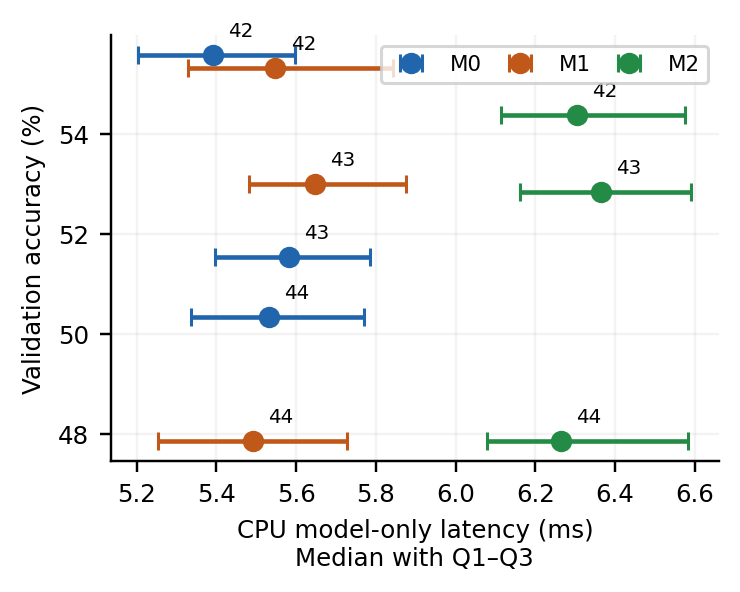
\includegraphics[width=\linewidth]{figures/accuracy_latency.png}
\caption{Accuracy versus CPU model-only latency. Labels identify student seeds. Horizontal bars are Q1--Q3 of 200 timed calls, not confidence intervals. M2 is slower than M1 in every paired seed on this machine.}\label{fig:tradeoff}
\end{figure}

\begin{table}[t]\centering\small
\begin{tabular}{lrrrr}\toprule
Model & Seed & Median & IQR & Peak RSS\\
 & & ms & ms & MiB\\\midrule
M0 & 42 & 5.391 & 0.392 & 1507.9 \\
M0 & 43 & 5.582 & 0.389 & 1591.1 \\
M0 & 44 & 5.532 & 0.435 & 1588.2 \\
M1 & 42 & 5.548 & 0.514 & 1589.4 \\
M1 & 43 & 5.648 & 0.394 & 1588.4 \\
M1 & 44 & 5.492 & 0.474 & 1589.3 \\
M2 & 42 & 6.305 & 0.461 & 1593.5 \\
M2 & 43 & 6.364 & 0.430 & 1594.1 \\
M2 & 44 & 6.265 & 0.505 & 1593.5 \\
\bottomrule\end{tabular}
\caption{Individual CPU runs. Peak RSS is whole-process peak, including imports, loading, conversion where applicable, and inference. It does not isolate inference-only memory.}\label{tab:lat}
\end{table}

\section{Ablation Study}
\subsection{Quantized components}
The Linear-only, embeddings-only and combined variants use the same selected M1 weights for each seed. Mean macro-F1 is 37.20, 37.10 and 36.96 respectively, compared with 37.28 for FP32 M1. Serialized states occupy 16.342, 5.894 and 4.675 MB respectively. The embedding table accounts for most of the observed storage reduction. Combined quantization gives the smallest state but the largest mean quality loss, 0.32 percentage points. Its prediction agreement with M1 is 96.56\%, 97.76\% and 98.71\% for seeds 42--44. Agreement with another model is not accuracy against ground truth.

\begin{figure}[t]\centering
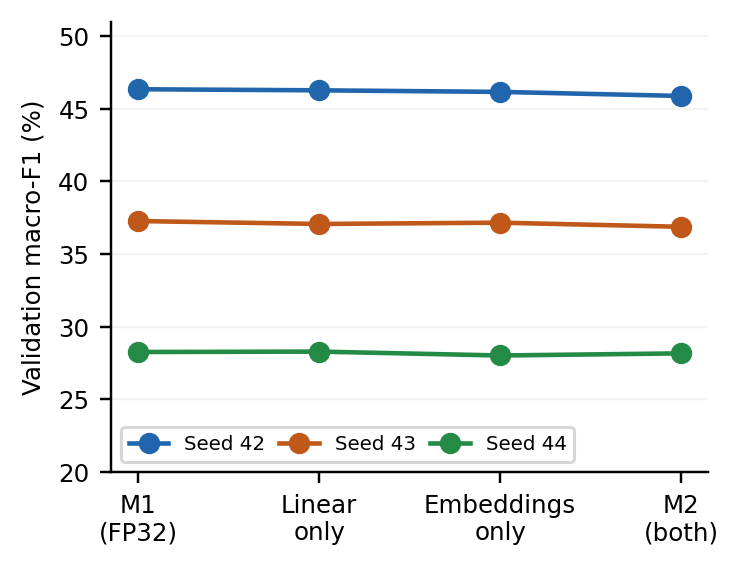
\includegraphics[width=\linewidth]{figures/quantization_ablation.png}
\caption{One-factor quantization ablation with paired seeds. The between-seed spread is much larger than the within-seed change induced by each quantization choice. Lines connect the same underlying student checkpoint.}\label{fig:ablation}
\end{figure}

\subsection{Temperature}
An additional $T=1$ distillation ablation holds the selected learning rate, loss mixing weight, update budget and all other student settings fixed. Table~\ref{tab:temperature} reports each trial's best validation checkpoint, not necessarily its final update.
\begin{table}[h]\centering\small
\begin{tabular}{lrr}\toprule
Seed & $T=1$ macro-F1 & $T=2$ macro-F1\\\midrule
42 & 44.21 & 46.34\\43 & 38.52 & 37.26\\44 & 30.13 & 28.25\\\midrule
Mean & 37.62 & 37.28\\\bottomrule\end{tabular}
\caption{Temperature ablation. $T=2$ was selected during the original validation search.}\label{tab:temperature}
\end{table}
Softening helps seed 42 but not seeds 43 or 44. The small mean difference does not establish a reliable temperature advantage. The selected $T=2$ model is not silently replaced after inspecting this exploratory ablation. Quantizing M0 remains an optional future comparison, not a completed result or a requirement added to this milestone.

\section{Efficiency Analysis}
Relative to M1, M2's mean serialized state is 73.38\% smaller, approximately 3.76 times smaller. This is a model-state storage result; it is not a 73\% reduction in the full application, parameters, MACs, peak RAM or training cost. The mean of per-seed median CPU latencies rises from 5.563 to 6.311 ms, an increase of 13.46\%. All three paired runs show this direction. Tokenization-inclusive medians are also retained in the CSV evidence; their measurement scope differs from the model-only plot.

Quantization overhead and limited opportunities to accelerate a tiny network are plausible explanations for slower inference. No operator-level profile was run, so these are hypotheses rather than established causes. The process peaks of roughly 1.5--1.6 GiB are dominated by a broader execution scope than the model state; this measurement does not demonstrate lower inference RAM. PyTorch's deprecation warnings were recorded, and the implementation is tied to the tested software version rather than silently migrated during the experiment.

Distillation does not shrink M0's architecture because both M0 and M1 already use the same BERT-Tiny student. It also requires Teacher training and target generation. The recovered selected Teacher record reports 1,718.94 seconds and a peak allocated GPU memory of 2,788.53 MiB. Its elapsed-time scope includes recovery I/O and excludes unsaved interrupted work; it is neither the total project GPU cost nor a fair isolated training-speed comparison. We report no energy or monetary savings.

\section{Preliminary Discussion}
The observed benefit is reduced model-state storage at a modest validation macro-F1 loss. Distillation does not provide the intended quality improvement, and quantization does not provide CPU speedup on the measured hardware. Consequently, M2 cannot be described as preserving a positive M1 advantage over M0: there is no positive mean advantage in this validation comparison. The predeclared test hypotheses remain unevaluated.

Seed sensitivity is substantial. Good Fit recall for M1 is 30.80\%, 32.87\% and 0.69\% across seeds 42--44; M2 yields 31.14\%, 30.45\% and 0.35\%. The seed-44 model nearly misses that class altogether. Confusion matrices and class reports expose this weakness even though overall accuracy is close to 48\%. The figures support caution about reliability and preclude an automated rejection claim. They do not alone establish why examples are misclassified.

Possible explanations include limited Teacher quality, sensitivity to initialization and data order, class imbalance, truncation and uncertain labels. These have not been experimentally isolated. After training, both authors independently assessed the same 90 training pairs and reviewed validation errors. These post-hoc reviews did not change the labels used for training. We report no numerical agreement statistic.

Repeated validation selection can produce optimistic development scores. Other limits include three student seeds, one Teacher, recurring CVs, uncertain data provenance and one CPU benchmark environment. This study does not demonstrate generalization to unseen candidates, calibration as a hiring probability, fairness across demographic groups or readiness for production deployment. Negative findings are retained rather than changing hypotheses after observing results.

\section{Connection to Senior}
The recruitment problem, terminology and workflow are reused from Senior. The compact classifier, validation protocol and efficiency measurements are new DL work. A successfully evaluated checkpoint could later be integrated into the backend as an advisory matching signal. It does not currently replace the planned API, implement practical verification, learn automatically from database storage, or justify autonomous rejection. Integration and a comparison against the actual Senior matching approach are future work.

\section*{AI Assistance and Author Review}
ChatGPT assisted with code restructuring, debugging, recovery checks, figures and report preparation. Earlier project materials disclose Claude assistance with paper checks, dataset research, workspace setup and planning. All experimental measurements come from the saved Colab runs. The authors conducted the independent label audit and qualitative error review.

\section*{Reproducibility and Submission Status}
The companion materials include the visible-code SetupFixed notebook, frozen split identifiers, protocol, validation results, CPU benchmark records, and figure reproduction script. Historical execution records are preserved separately from the clean notebook.

Project repository: \url{https://github.com/RAWANKHOJAH/HireMind-DL}. The Assignment 3 materials are organized in \texttt{assignment\_3/}. Held-out test evaluation is reserved for the final milestone.

\clearpage
\balance
\begin{thebibliography}{9}
\bibitem[Bondarenko et al.(2021)]{bondarenko} Yelysei Bondarenko, Markus Nagel, and Tijmen Blankevoort. 2021. Understanding and Overcoming the Challenges of Efficient Transformer Quantization. \emph{EMNLP}, pages 7947--7969. DOI: 10.18653/v1/2021.emnlp-main.627.
\bibitem[Devlin et al.(2019)]{bert} Jacob Devlin, Ming-Wei Chang, Kenton Lee, and Kristina Toutanova. 2019. BERT: Pre-training of Deep Bidirectional Transformers for Language Understanding. \emph{NAACL-HLT}, pages 4171--4186.
\bibitem[Gan et al.(2024)]{gan} Chengguang Gan, Qinghao Zhang, and Tatsunori Mori. 2024. Application of LLM Agents in Recruitment: A Novel Framework for Automated Resume Screening. \emph{Journal of Information Processing}, 32:881--893. DOI: 10.2197/ipsjjip.32.881.
\bibitem[Hinton et al.(2015)]{hinton} Geoffrey Hinton, Oriol Vinyals, and Jeff Dean. 2015. Distilling the Knowledge in a Neural Network. \emph{arXiv:1503.02531}.
\bibitem[Jiao et al.(2020)]{tinybert} Xiaoqi Jiao, Yichun Yin, Lifeng Shang, Xin Jiang, Xiao Chen, Linlin Li, Fang Wang, and Qun Liu. 2020. TinyBERT: Distilling BERT for Natural Language Understanding. \emph{Findings of EMNLP}, pages 4163--4174. DOI: 10.18653/v1/2020.findings-emnlp.372.
\bibitem[Sanh et al.(2019)]{distilbert} Victor Sanh, Lysandre Debut, Julien Chaumond, and Thomas Wolf. 2019. DistilBERT, a distilled version of BERT: smaller, faster, cheaper and lighter. \emph{EMC$^2$ Workshop at NeurIPS}. arXiv:1910.01108.
\bibitem[Turc et al.(2019)]{turc} Iulia Turc, Ming-Wei Chang, Kenton Lee, and Kristina Toutanova. 2019. Well-Read Students Learn Better: On the Importance of Pre-training Compact Models. \emph{arXiv:1908.08962}.
\bibitem[Zafrir et al.(2019)]{q8} Ofir Zafrir, Guy Boudoukh, Peter Izsak, and Moshe Wasserblat. 2019. Q8BERT: Quantized 8Bit BERT. \emph{EMC$^2$ Workshop at NeurIPS}. DOI: 10.1109/EMC2-NIPS53020.2019.00016.
\bibitem[Zhang et al.(2020)]{ternary} Wei Zhang, Lu Hou, Yichun Yin, Lifeng Shang, Xiao Chen, Xin Jiang, and Qun Liu. 2020. TernaryBERT: Distillation-aware Ultra-low Bit BERT. \emph{EMNLP}, pages 509--521. DOI: 10.18653/v1/2020.emnlp-main.37.
\end{thebibliography}
\end{document}
